\begin{figure}
  \begin{center}
  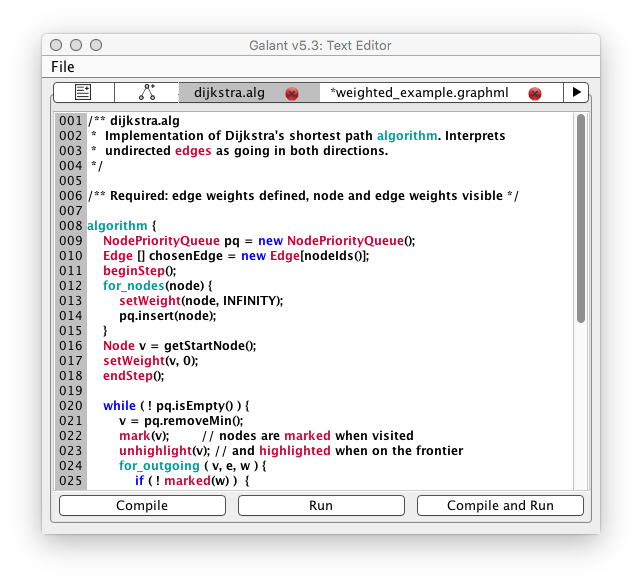
\includegraphics[scale=0.45]{X-dijkstra_text}

  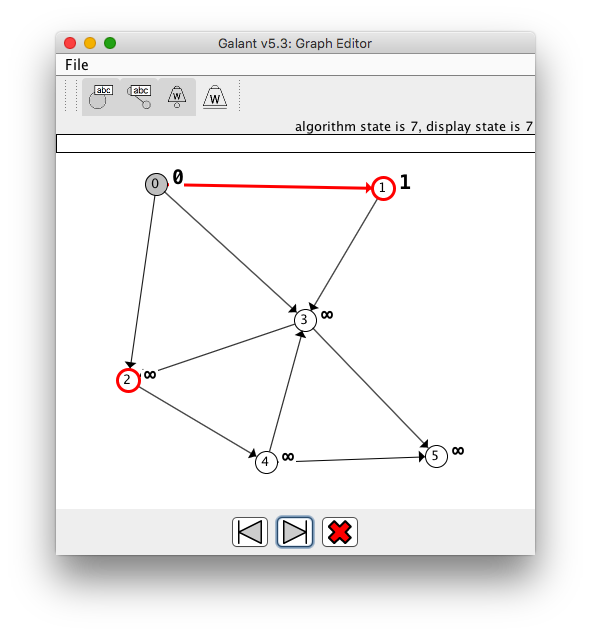
\includegraphics[scale=0.45]{X-dijkstra_running}
  \end{center}

  \caption{The text and graph windows when an algorithm is running. The text
    window is at the top -- it has buttons for the user to select
    whether to compile the algorithm, run it (if already compiled) or do
    both. The graph window in the middle of algorithm execution is at
    the bottom.}
  \label{fig:dijkstra_running}
\end{figure}

% [Last modified: 2016 12 22 at 22:25:28 GMT]
